% drawtizk
% drawtizk


\usepackage{tikz}
\usepackage{pgffor}%可以使用foreach的包
\usepackage{ifthen}%可以使用ifthenelse的包,还能使用whiledo

\begin{document}
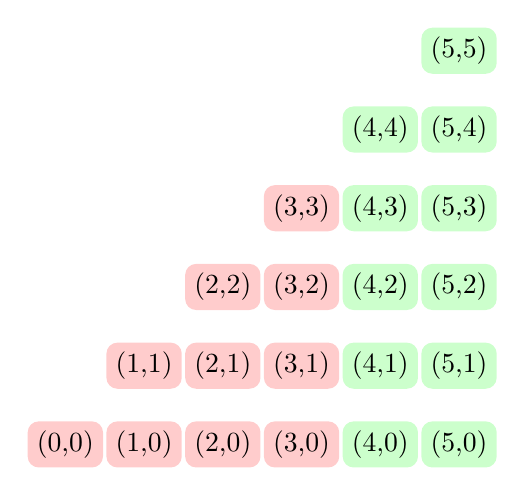
\begin{tikzpicture}
    \foreach \i in {0,...,5}{
        \foreach \j in {0,...,\i}{
            \ifthenelse{\i > 3}{%if成立
                \node[fill = green!20,rounded corners]at (\i,\j) {(\i,\j)};
            }{%if不成立
                \node[fill = red!20,rounded corners]at (\i,\j) {(\i,\j)};
            }
        }
    } 
\end{tikzpicture}
